
\subsection{Setting 2: Function Selection}

In this section, we study the ability of our method to recover the true function.
We use RBF kernels on each group by setting kernel bandwidths
for each dimension as same as above.
Extending the generative model in \cite{ravikumar09spam}, 
we generate observations from the following
50-dimensional additive model:
\begin{align*}
	y_i =& f_1(x_{i1}) + f_2(x_{i2}) + f_3(x_{i3}) + f_4(x_{i4}) + \\
&f_1(x_{i5}x_{i6}) + f_2(x_{i7}x_{i8}) + \\
&f_3(x_{i9}x_{i10}) + f_4(x_{i11}x_{i12}) + \epsilon_i \\
f_1(x) =& -2\sin(2x), f_2(x) = x^2 - \frac{1}{3}, \\
f_3(x)=& x-\frac{1}{2}, f_4(x) = e^{-x} + e^{-1} - 1
\end{align*}
with noise $\epsilon_i \sim \mathcal{N}(0,1)$.
Thus, 46 out of 50 individual features are irrelevant, and
1221 out of 1225 pairwise features are irrelevant.

We plot the solution path for two independent datasets, 
with $n=200$ and $n=600$ observations, respectively.
Our results are shown in Figure \ref{fig:n200}. 

\begin{figure}
\centering
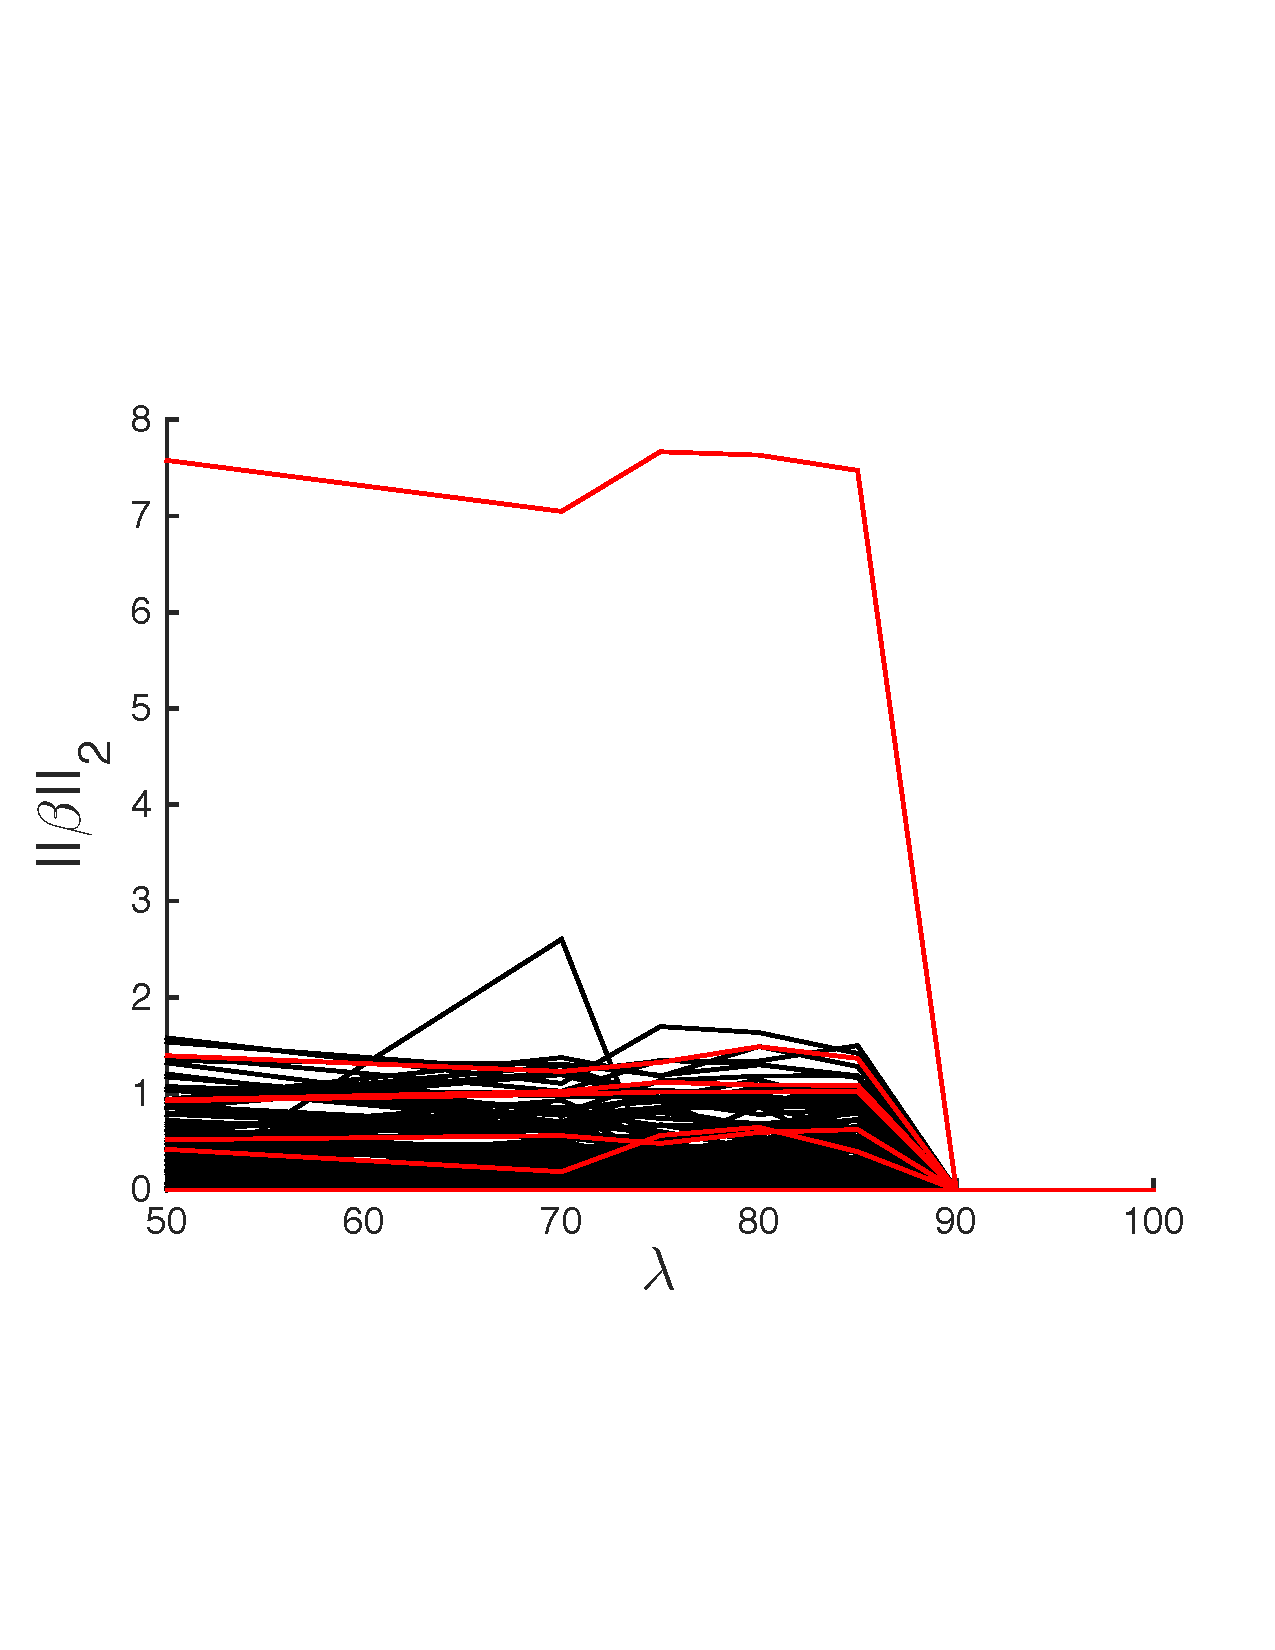
\includegraphics[width=3.4in]{figs/solnpath200.pdf}
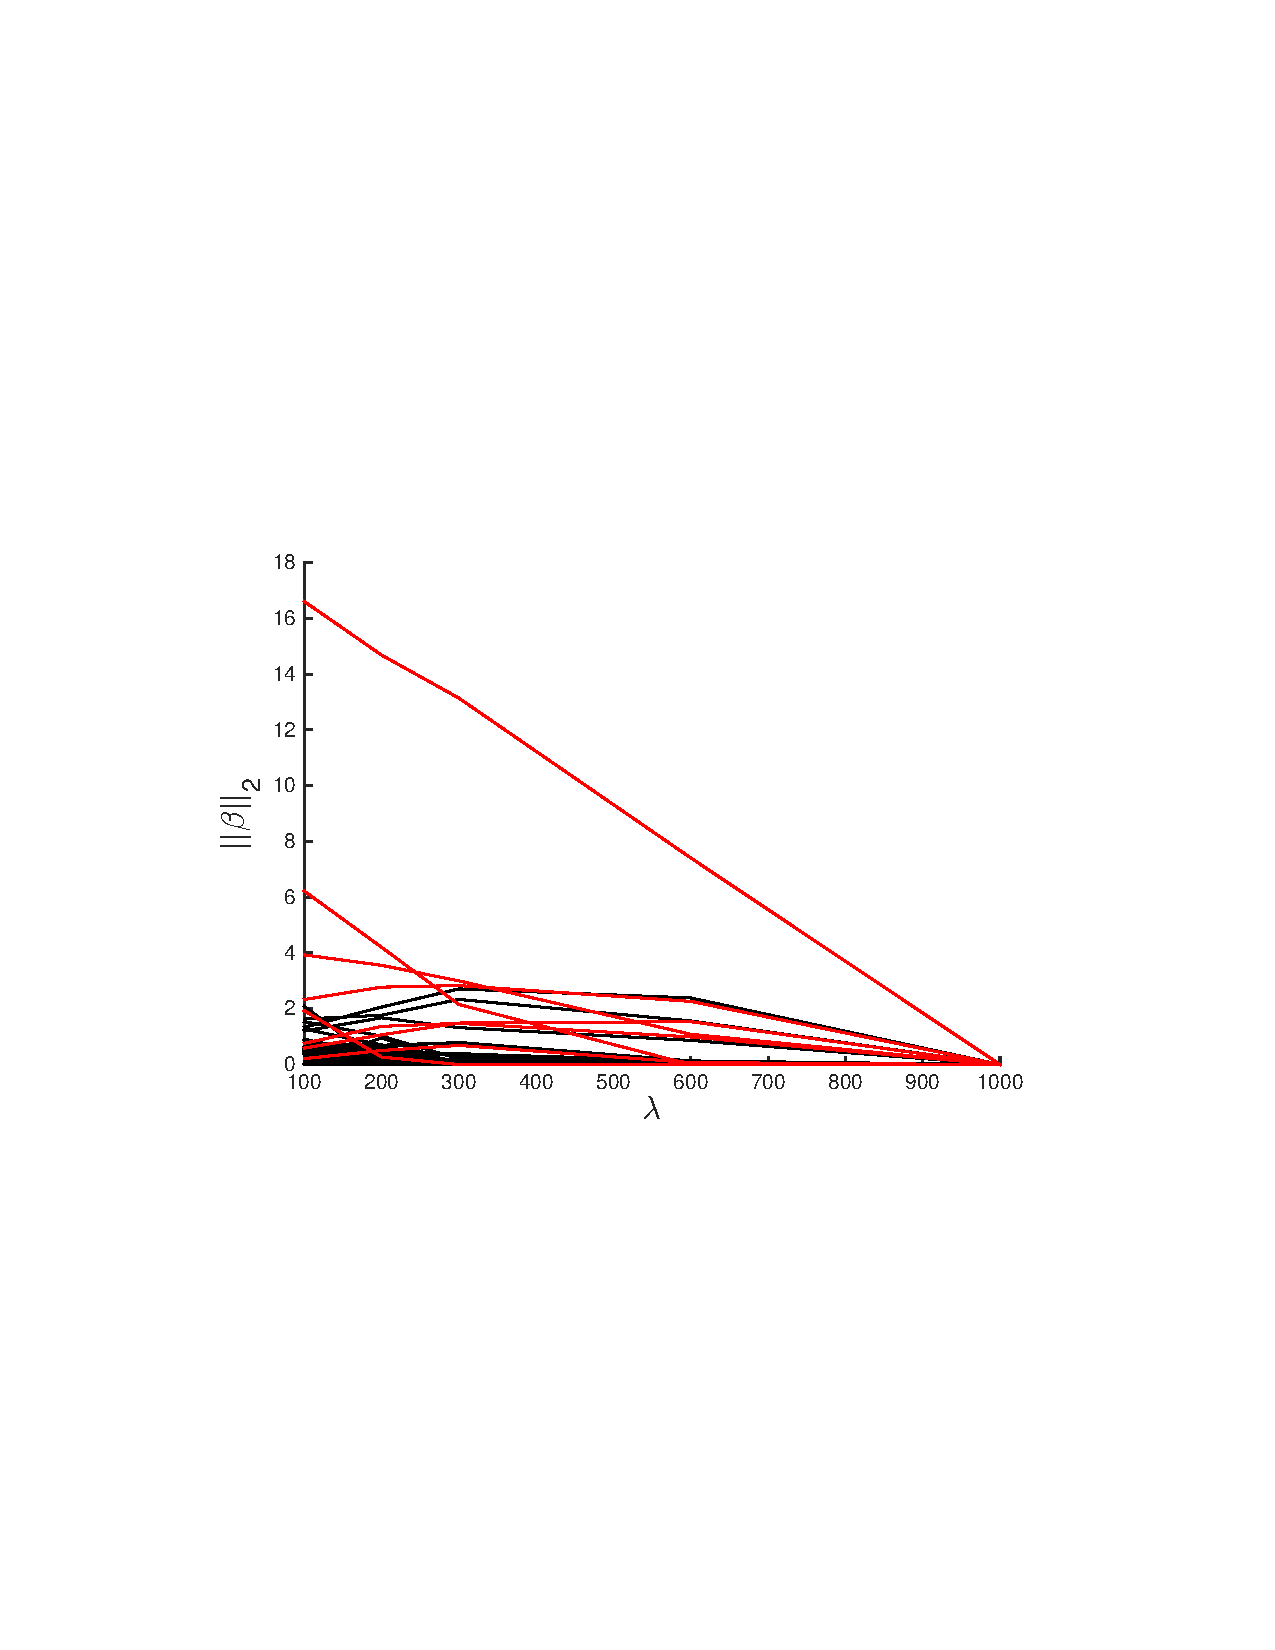
\includegraphics[width=3.2in]{figs/solnpath600.pdf}
\vspace{\imcaptionspace}
\caption[]{\small Solution path with $n=200$ samples (above) and
$n=600$ (below). The $x$-axis shows the regularization parameter,
while the $y$-axis plots the $\ell_2$-norm of all $\beta_j$ }
\vspace{\imtextspace}
\label{fig:n200}
\end{figure}

